\documentclass[a4paper,10pt]{article}
\usepackage{latexsym}
\usepackage[american]{babel}
\usepackage{lmodern}
\usepackage[utf8x]{inputenc}
\usepackage[T1]{fontenc}
\usepackage{longtable}
%\usepackage[dvips]{graphicx}
\usepackage{graphicx}

%\usepackage[pdftex]{hyperref}
\usepackage{hyperref}
\usepackage{amsmath}  % for equation environment
\usepackage{enumitem} % nolistsep to reduce list spacing

\usepackage{parskip} % no indentation in paragraphs

%opening
\title{Automated test generation for {\tt ctsa}}
\author{@hgfernan}
\frenchspacing

\pagestyle{myheadings}

\markboth{Automated test generation for {\tt ctsa}}
         {Automated test generation for {\tt ctsa}}

\addtolength{\hoffset}{-1,5cm}
\addtolength{\textwidth}{+3.5cm}

\addtolength{\voffset}{-1,2cm}
\addtolength{\marginparwidth}{-0,5cm}
\addtolength{\textheight}{+3.5cm}

% \linespread{1.5}


\begin{document}

\maketitle

\tableofcontents

\begin{abstract}
A routine for the automated test generation for the statistical
library {\tt ctsa} is outlined. It envolves the generation of
simple tasks of model fitting and prediction using {\tt ctsa},
compared with equivalent code in the Python libraries
{\tt pmdarima} and {\tt statsmodels}, and in the R library
{\tt forecast.}
\end{abstract}

\section{Motivation}
\label{sec:motiv}

{\em Why using a test database and automatic generation of
tests, instead of the handcrafted tests ?}

\section{Introduction}
\label{sec:intro}

{\em Overview of the project}

\section{Tables}
\label{sec:tables}

Since the automated test generation is based on a database, here
follows a description of the database to be used.

It has a mixed relational and document architecture: the main
tables follow a conventional relational structure, but the
parameters and test results are stored as JSON values. That's for
pragmatic reasons: the parameters and test results are varied and
have different structures. That could be easily mapped to a
relational database structure, but it would be too laborious and
cumbersome.

For instance: an $ARIMA$ model will have three basic parameters,
while a $SARIMA$ model will have 7 basic parameters.

As such, test parameters and results will be stored as JSON
objects encoded as strings, and dealt with by classes specialized
in their content. There will be a class for each one of the
models, that will be able to unpack and allow the use of the
information in those JSON values.

\begin{figure}[h]
    \centering
    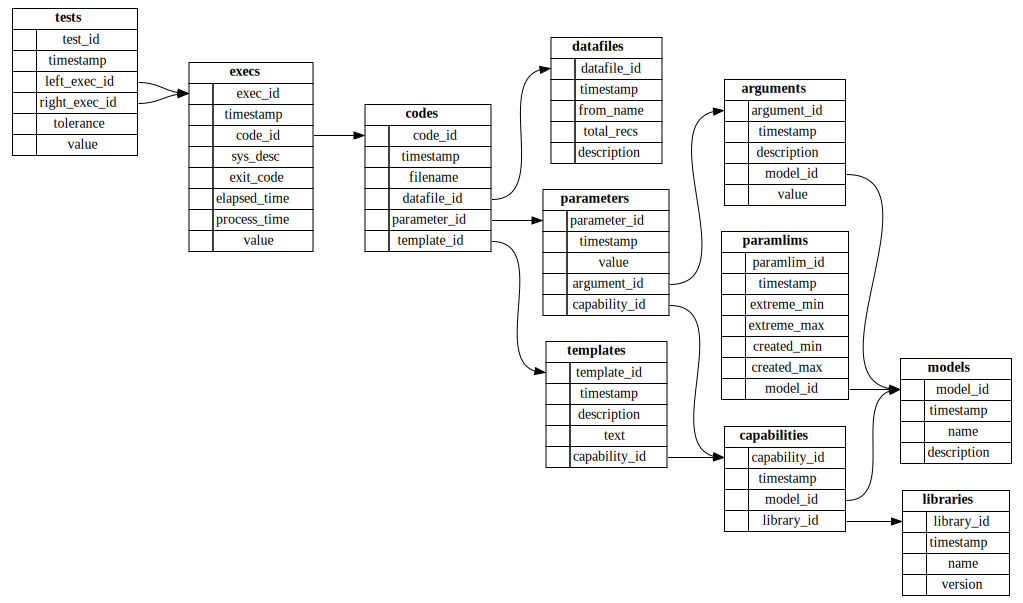
\includegraphics[scale=0.35]
        {../img/schema.jpg}
    \caption{Database used for automated test generation}
    \label{fig:schema}
\end{figure}

A short description of the data base structure displayed in Figure
\ref{fig:schema} can be:

\begin{enumerate}
    \item \label{itm:models}
        The most central table is {\tt models}m that contains
        the name of all statistical models in use.

        It is related to 3 other tables: {\tt arguments} (item
        \ref{itm:arguments}), {\tt capabilities} (item
        \ref{itm:capabilities}), and {\tt paramlims} (item
        \ref{itm:paramlims});

    \item \label{itm:libraries}
        The second central table is {\tt libraries}. It contains
        the names of the libraries that shall be used in the tests.

        All libraries in use -- that is {\tt ctsa},
        {\tt forecast}, {\tt pmdarima}, and {\tt statsmodels} --
        are available in just one language, be it C, Python or R.
        Therefore there's currently no need to add a language field
        in this table.

        Another possible lack of information will be the partial
        support of a statistical model in one or more of the
        libraries, but for now its solution will be postponed;

    \item \label{itm:capabilities}
        Another important table is {\tt capabilities}, that's a
        relationship between {\tt models} (item \ref{itm:models})
        and {\tt libraries} (item \ref{itm:libraries}); that is:
        it informs what statistical models are supported by each
        library.

        This table guides the creation of code {\tt templates}
        (item \ref{itm:templates}) for each language and library,
        as well as the adaptation of statistical {\tt arguments}
        (item \ref{itm:arguments}) for each library, in the form
        of {\tt parameters} (item \ref{itm:parameters});

    \item \label{itm:datafiles}
        The table {\tt datafiles} contains a list of data files
        specially prepared for the tests: they contain only a time
        series, in the fields {\tt index} and {\tt value}, to
        ease the creation of tests. As such they don't have a
        specific name: they're named with the {\tt datafile\_id}
        and the extension ``{\tt .csv}''. For instance, the 1st
        file registered in this table will be named
        ``{\tt 0001.csv}''.

        The table field {\tt from\_name} relates this adapted data
        file to the original data where the data was obtained;

    \item \label{itm:arguments}
        The table {\tt arguments} contains values of elements
        of the statistical {\tt models} (item \ref{itm:models}),
        without any concern to its implementation in the
        {\tt libraries} (item \ref{itm:libraries});

    \item \label{itm:parameters}
        The table {\tt parameters} contains the adaptation of the
        table {\tt arguments} (item \ref{itm:arguments}) to each
        implementation of one of the {\tt models}) (item
        \ref{itm:models}) of the codes of the  {\tt libraries}
        (item \ref{itm:libraries}).

        That adaptation is done via the field {\tt value}.

        This table refers the {\tt capabilities} (item
        \ref{itm:capabilities}) to

        It is used to create a relate {\tt models} and
        {\tt libraries};

    \item \label{itm:templates}
        The table {\tt templates} contains codes templates to
        each one of the library {\tt capabilities}
        (item \ref{itm:capabilities}) -- that is all the
        statistical {\tt models} (item \ref{itm:models}) that all
        {\tt libraries} (item \ref{itm:libraries}) implement.

        A template is conceptually an open structure with holes
        where the {\tt parameters} (item \ref{itm:parameters})
        and the {\tt datafiles} (item \ref{itm:datafiles}) will
        be filled in. A template is also a fragment of source
        code where just these two informations are missing;

    \item \label{itm:codes}
        The table {\tt codes} contains the source codes generated
        by filling in each one of the {\tt templates} (item
        \ref{itm:templates}) with one of {\tt datafiles} (item
        \ref{itm:datafiles}) and one of {\tt parameters}
        (item \ref{itm:parameters}).

        The table {\tt codes} a tiny of the table {\tt templates},
        but it's an important one, since makes more concrete this
        filling of a template.

        Another point to make matters more clear is that the
        name of a code file (contained in the field
        {\tt filename}) won't be simply the transcription of the
        field {\tt code\_id} and an extension, but will refer to
        the field {\tt name} of the corresponding row in
        {\tt model} (item \ref{itm:models}), of the {\tt name} of
        used row in {\tt libraries}, the {\tt parameter\_id}
        of the parameter used, and the {\tt datafile\_id} of the
        data file used in it.

        That is: the simple naming used in {\tt datafiles} (item
        \ref{itm:datafiles}) won't be used here.

        For instance: if a {\tt codes} row with {\tt code\_id}
        of $15$, uses a C code template of library {\tt ctsa},
        its filename would ``{\tt 0015.c}''. But if it uses the
        $AR$ model implementation of {\tt ctsa}, uses the 1st row
        of parameters, and the {\tt datafile\_id} of $23$, its
        extended name will be ``{\tt ar\_ctsa\_p0001\_d0023.c}''

    \item \label{itm:paramlims}
        The table {\tt paramlims} contains the valid range of
        each parameter of a given model from the table
        {\tt models} (item \ref{itm:models}), from the value
        in the field {\tt extreme\_min} to the value
        {\tt extreme\_max}, inclusive.

        The execution of all codes -- as contained in the table
        {\tt execs} (item \ref{itm:execs}) -- can take some time;
        therefore the parameters really used to create code files
        for all libraries will be kept in the closed interval of
        the field pair
        $[${\tt created\_min}, {\tt created\_max}$]$;

    \item \label{itm:execs}
        The table {\tt execs} contains a history of the executions
        of a given code. Its only link is with the table
        {\tt codes} (item \ref{itm:codes}).


        The fields in {\tt execs} document the execution of a
        given code, identified by its {\tt code\_id}. The field
        {\tt sys\_desc} should contain the description of the
        machine where code was run, {\tt exit\_code} is the value
        returned by the execution of the code. The time of
        execution is measured by {\tt elapsed\_time} (the
        difference between the time the execution was started and
        the time it was finished), and {\tt process\_time} is the
        time of the CPU that was effetively used.

        The field {\tt value} contains both the parameters used in
        to start the program, and the result it obtained. It
        contains the information presented as the summary of the
        fitting of the model to  the data, and the result of the
        forecasting of a few time steps, both as the value
        obtained, and its deviation.

        That information is formatted as a JSON encoded string,
        due to the variety of parameters of each statistical
        model, as well as the variety of their measures of fitting.

    \item \label{itm:tests}
        Finally, the table {\tt tests} is a comparison between two
        different executions of the same data, aka
        {\tt datafile\_id}, the same statistical model and the
        same model arguments; that is the same {\tt argument\_id}.
        One is called {\tt lef\_exec\_id} and the other is
        {\tt right\_exec\_id}.

        A test allows two different versions of the same library
        to be compared for the same model and arguments. Or two
        different libraries with the same model and arguments.

        The comparison can use the statistical or the results of
        the physical execution, like the process time or the
        exit code.
\end{enumerate}


% In a few words, the algorithm to generate tests follow this way:
%
% \begin{enumerate}
%     \item The table {\tt paramlims} (on the upper left corner of
%         Figure \ref{fig:schema}) is used to select a sequence of
%         parameters for each model, according to the limits present
%         in the fields {\tt extreme\_min} and {\tt extreme\_max}.
%         They are stored in the table {\tt params} to be detailed
%         below.
%
%         Not all parameters are generated, and the range of the
%         parameters created up to the moment are saved in the
%         fields {\tt created\_min} and {\tt created\_max}.
%
%         The field {\tt timestamp} contains the last alteration
%         of any or all values in the range {\tt created\_min} and
%         {\tt created\_max} for its corresponding {\tt model};
%
%     \item The list of data files available (stored in the folder
%         {\tt data/}) are listed and the original name and place of
%         each one is contained in the field {\tt filename} of the
%         table {\tt datafiles}. In this table the date of each file
%         inclusion is recorded in the field {\tt timestamp}. The
%         field {\tt total\_recs} of the same table contain the
%         number of records of each file. The field
%         {\tt description} can be used to introduce details of the
%         file: its origin, the transformations used to generate it,
%         etc.
%
%     \item \label{itm:codes}
%         There are simple templates for each model, and they're
%         used to generate a single file for each of the elements of
%         the cartesian product between the allowed range of
%         {\tt params} for each model, and the data files in
%         {\tt datafiles}.
%
%         This process is replicated for each of the languages in
%         use (C, Python, and R) and their corresponding libraries
%         {\tt ctsa}, {\tt pmdarima} and {\tt statsmodels}, and
%         {\tt forecast}. Those results are stored in the table
%         {\tt codes}, and only the programming language is stored
%         there, as just a single library will be used for each
%         case.
%
%         After the testing {\em per se}, a fragment of the code
%         stores in a CSV file the parameters, the calculated
%         results and the elapsed and processing times, as well
%         other information needed, as described in item
%         \ref{itm:execs};
%
%     \item \label{itm:execs}
%         The codes generated are then run, as the resources in
%         processing hardware and time allow for it.
%
%         The execution results are stored in the table
%         {\tt tables}, and they are retrieved from a CSV file
%         that each execution generate, as described in the item
%         \ref{itm:codes}.
%
%         This table contains the field {\tt timestamp} that will
%         inform when the execution was started. The field
%         {\tt code\_id} refers to the source code that was used.
%         The field {\tt sys\_desc} should contain a description
%         of the hardware that was used to run the code, as precise
%         as possible. Even though precision in the results is the
%         main purpose of this suite of tests, a marginal point is
%         the processing speed of each implementation. Of course,
%         that comparison would be meaninful only if the execution
%         scenarios of each benchmark participant were kept
%         constant.
%
%         The table also contains the fields {\tt elapsed\_time},
%         that contains the clock time spent for the execution, and
%         {\tt proc\_time} that contains the time spent using the
%         processor or processors available in the hardware.
%
%         Finally, the field {\tt value} is a JSON value encoded as
%         a string that contain two data structures, named
%         {\tt params}, where a copy of the model parameters is
%         stored, and {\tt results}, where a copy of the numerical
%         parameters is stored.
%
%         There's some space for the results of a model -- for
%         instance, the number of time steps forecasted --, but
%         the intelligence to handle that variation will be kept in
%         the class that handles each results;
%
%     \item \label{itm:tests}
%         Finally the table {\tt tests} holds what could be
%         considered a test, actually a comparison between two
%         executions, or fields in the table {\tt execs}.
%
%         The field {\tt timestamp}, as usual, contains the
%         information of the time when the comparison was started.
%         The field {\tt left\_exec\_id} identifies the execution
%         that will be compared against other execution, represented
%         by the field {\tt right\_exec\_id}. Typically, it will be
%         an execution of a program based upon {\tt ctsa} and
%         another based upon one of its equivalent libraries using R
%         or Python.
%
%         And it is recommended that the comparisons are made only
%         between two executions in the same hardware, described
%         by {\tt sys\_desc}, as mentioned in the item
%         \ref{itm:execs}.
%
%         The comparison are executed against the value given in the
%         field {\tt tolerance}. The relative deviation $d_{rel}$
%         is calculated for each parameter as
%         \begin{equation*}
%             d_{rel} = \frac{ |p_{right} - p_{left}| }{p_{right}}
%         \end{equation*}
%         And a test passes when $d_{rel} \leq tolerance$; otherwise
%         it fails.
%
%         The field {\tt value} is a JSON value encoded as a
%         structure, that contains two data structures, one named
%         {\tt params}, where a copy of the model parameters is
%         stored, and another named {\tt results}, that contains for
%         each result a triplet with the numeric value of the result
%         of the left test, the value of the result of the right
%         test, and string ``{\tt pass}'' if the test passed, or
%         ``{\tt fail}'' if the test failed.
%
% \end{enumerate}

\section{Software design}
\label{sec:design}

{\em High level specification of the softwares and their use.}

\section{Examples by hand}
\label{sec:by_hand}

{\em Worked examples of the database and software use.}

\section{Implementation}
\label{sec:impl}

{\em A shiplog reporting details of the system development, and
possible deviations from the specification in the section
\nameref{sec:design}}.

\end{document}
